\documentclass[tikz, border=15pt]{standalone}
\usepackage{tikz}
\usetikzlibrary{calc, arrows.meta}

\begin{document}
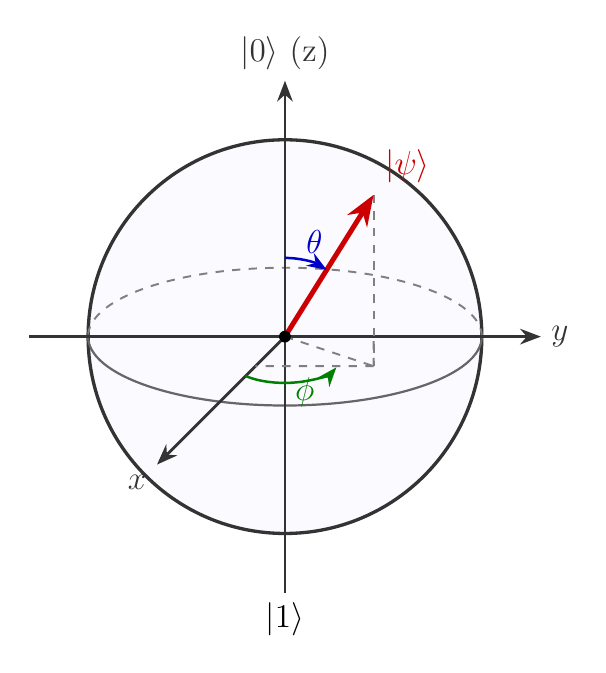
\begin{tikzpicture}[
    scale=2.5,
    >=Stealth,
    axis/.style={->, line width=1.0pt, color=black!80},
    vector/.style={->, line width=1.8pt, color=red!80!black},
    dashedline/.style={dashed, color=black!50, line width=0.7pt}
]

    % Sphere background fill & main circle
    \fill[blue!5, opacity=0.4] (0,0) circle (1);
    \draw[line width=1.2pt, color=black!80] (0,0) circle (1);

    % Equator (ellipse)
    \draw[line width=0.8pt, color=black!60] (-1,0) arc (180:360:1 and 0.35);
    \draw[dashedline] (1,0) arc (0:180:1 and 0.35);

    % Axes
    % Z axis
    \draw[axis] (0,-1.3) -- (0,1.3) node[above, font=\large] {$|0\rangle$ (z)};
    \node[below, font=\large] at (0,-1.3) {$|1\rangle$};

    % Y axis
    \draw[axis] (-1.3,0) -- (1.3,0) node[right, font=\large] {$y$};

    % X axis (projected forward)
    \draw[axis] (0,0) -- (-0.65,-0.65) node[below left, font=\large] {$x$};

    % State Vector |psi> coordinates
    \coordinate (O) at (0,0);
    \coordinate (P) at (0.45, 0.72); % Position of |psi>
    \coordinate (Pproj) at (0.45, -0.15); % Projection on xy plane

    % Projection lines
    \draw[dashedline] (O) -- (Pproj);
    \draw[dashedline] (P) -- (Pproj);
    \draw[dashedline] (Pproj) -- (0.45, 0);
    \draw[dashedline] (Pproj) -- (-0.15, -0.15);

    % Vector |psi>
    \draw[vector] (O) -- (P) node[above right, font=\large] {$|\psi\rangle$};

    % Angle theta (between Z and P)
    \draw[->, line width=0.9pt, color=blue!80!black] (0,0.4) arc (90:58:0.4);
    \node[color=blue!80!black, font=\large] at (0.15, 0.48) {$\theta$};

    % Angle phi (between X axis line and Pproj)
    \draw[->, line width=0.9pt, color=green!50!black] (-0.2, -0.2) arc (225:340:0.28 and 0.12);
    \node[color=green!50!black, font=\large] at (0.1, -0.28) {$\phi$};

    % Origin dot
    \fill[black] (O) circle (0.03);

\end{tikzpicture}
\end{document}
